\documentclass[a4paper, 11 pt, article, accentcolor=tud7b]{tudreport}

\usepackage[utf8]{inputenc}
\usepackage{amsmath}
\usepackage{placeins}
\usepackage{tabularx}
\usepackage{subcaption}

\title{CNuVS Exercise 9}
\author{Nils Rollshausen, Daniel Drodt}
\subtitle{Nils Rollshausen, Daniel Drodt}

\begin{document}
	\maketitle
	\section{TCP Congestion control}
	\subsection*{a) Congestion control vs flow control}
	Flow control intends to protect the receiver from overload while congestion control protects the network. TCP specifically uses a window-based approach to congestion control.
	  
	\subsection*{b) Congestion window}
	The amount added to the congestion window with each ack is given as $inc = MSS \cdot \frac{MSS}{window}$. So, on the first acknowledgement, we increment the window by $1320 \cdot \frac{1320}{13200} = 132$ bytes to $13332$ bytes. On the second ack, we increment by $1320 \cdot \frac{1320}{13332} = 130.69$ byte to a new congestion window of $13462.69$ byte.
	
	\subsection*{c) Slow start}
	After establishing a connection or pausing the connection when congestion is detected, it would take a long time for TCP to incrementally adjust the congestion window to its proper value. To speed this process up, the congestion window is increased exponentially (as opposed to linearly in the regular congestion avoidance phase) until the desired window size is reached (half the previous window if a packet loss has been detected) or a packet is lost.
	
	\section{Three-Way-Handshake}
	
	\subsection*{a) Handshake}
	The three-way-handshake consists of the initiating party sending a SYN packet to the receiving party. The receiving party responds to the SYN request with a SYN-ACK packet acknowledging the receipt of the SYN request. Finally, the initiating party acknowledges the receipt of the SYN-ACK with an ACK packet.
	
	\subsection*{b) TCP Segment}
	
	In addition to the fields already given, the TCP header contains the following values:
	
	\begin{table}[h]
	  \centering
	  \begin{tabular}{|l|l|}
	    \hline
	    Source port & 0x076c \\ \hline
	    Destination port & 0x07cd \\ \hline
	    Data offset & 0x5 \\ \hline
	    Checksum & 0x3c8f \\ \hline
	  \end{tabular}
	  \caption{Remaining TCP header fields}
	\end{table}
	
	The application data is \verb|0x4e6f 7274 6865 726e 204c 6967 6874 7300|. The checksum is calculated as the inverse two's-complement sum as follows: 
	
	\begin{align*}
	  0xFFFF - (&0x076c + 0x07cd + 0x0000 + 0x1337 + 0x0000 + 0x0000 \\
	            &+ 0x5020 + 0x5000 + 0x0000 + 0x0000 + 0x4e6f + 0x7274 \\
	            &+ 0x6865 + 0x726e + 0x204c + 0x6967 + 0x6874 + 0x7300) \\
	          = &0xFFFF - 0xC370 = 0x3C8F
	\end{align*}
	
	\newpage
	
	\subsection*{c) TCP header fields}
	
	\begin{table}[h]
	  \centering
	  \begin{tabularx}{\linewidth}{|l|X|}
	    \hline
	    Source port & The port from which the packet is sent \\ \hline
	    Destination port & The port to which the packet is sent \\ \hline
	    Sequence number & Sequence number of the packet, corresponds to bytes already sent \\ \hline
	    Acknowledgement number & If the ACK flag is set, this acknowledges the receipt of all bytes up to the acknowledgement number \\ \hline
	    Data offset & The length of the header in 32 bit words, used to determine where the payload starts \\ \hline
	    Reserved & Reserved bits intended for future extensions of the protocol \\ \hline
	    URG & Indicates that the Urgent Data Pointer field is valid and should be considered \\ \hline
	    ACK & Indicates that the acknowledgement number is valid \\ \hline
	    PSH & Indicated that received data should be pushed to the receiving process immediately \\ \hline
	    RST & Resets the connection \\ \hline
	    SYN & Indicates a connection request \\ \hline
	    FIN & Indicates a connection termination \\ \hline
	    Window Size & The amount of bytes the sender of the packet is currently willing to receive, starting at the value in the acknowledgement field \\ \hline
	    Checksum & The 16bit twos-complement checksum over the entire packet \\ \hline
	    Urgent Pointer & If URG is set, this indicates that the first n bytes from the message start are urgent \\ \hline
	  \end{tabularx}
	  \caption{TCP header fields}
	\end{table}
	
	\subsection*{d) Retransmission}
	\begin{figure}[h]
    \begin{subfigure}[b]{0.3\textwidth}
      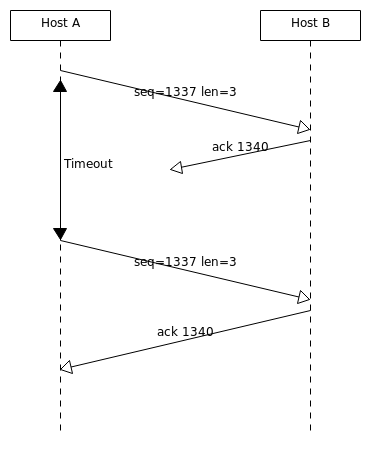
\includegraphics[width=\textwidth]{retrans1.png}
      \caption{Lost ACK}
      \label{fig:1}
    \end{subfigure}
    %
    \begin{subfigure}[b]{0.3\textwidth}
      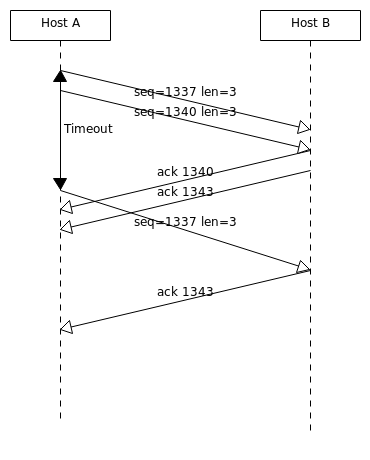
\includegraphics[width=\textwidth]{retrans2.png}
      \caption{Premature Timeout}
      \label{fig:2}
    \end{subfigure}
    %
    \begin{subfigure}[b]{0.3\textwidth}
      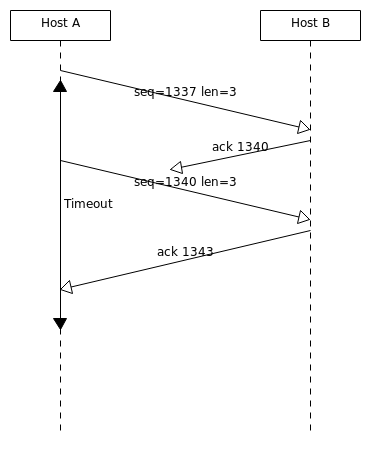
\includegraphics[width=\textwidth]{retrans3.png}
      \caption{Cumulative ACK}
      \label{fig:2}
    \end{subfigure}
  \end{figure}
	When an ACK packet is lost, the sender would, after a timeout, consider the packet whose acknowledgement got dropped to be lost and re-send it. The receiver recognizes the re-sent packet as a duplicate, discards it, and responds with an up-to-date acknowledgement.
	
	\FloatBarrier
	
	\section{RED, State Chart \& Nagle}
	
	\subsection*{a) Random Early Detection}
	Random Early Detection is necessary for routers and other network equipment to signal to end nodes that they are running close to their maximum capacity. As the routers should be agnostic to the choice of transport protocol, there is no protocol-inherent mechanism for them to communicate their capacity. As a solution, routers communicate implicitly by randomly dropping packets when running close to maximum load to reduce the network load before actually running completely out of capacity, which would lead to heavy congestion.
	
	\subsection*{TIME\_WAIT and ESTABLISHED}
	The TIME\_WAIT state is used by the party terminating a connection to ensure that the other party was able to terminate the connection properly (i.e. it received the acknowledgement to its FIN). A duplicate received FIN in this state indicates that the previous ACK was lost and should be retransmitted. After a sufficient amount of time passes, it can be assumed that no such duplicate FIN will arrive and the remote party was able to terminate the connection. \\ \medskip
	The ESTABLISHED state is the normal state of a TCP connection in which both parties have established the connection and are able to send and receive data.
	
	\subsection*{c) Nagle's Algorithm}
	Nagle's Algorithm deals with the problem network congestion caused by acknowledging small amounts of data and thus creating very high network overhead for comparatively little data. It states that data should only be sent if either the amount of data to send is larger or equal to the maximum segment size or there is no unacknowledged data packet still in-flight to the receiver. Using this algorithm, non-full packets are only sent when it is assumed that the receiver is currently idle.
	
	\end{document}
